\section{System Model}
\label{sec:model}
In this section, we elaborate the model of edge computing networks with random job arrivals, uploading latency and computation time, as well as the signaling mechanism with periodic broadcast.
% as well as the signaling model with periodic broadcast which introduce the job dispatching actions making under partially observable system state at each AP.
%----------------------------------------------------------------------------------------%
\subsection{Network Model}
% \begin{figure*}[htp!]
%     \centering
%     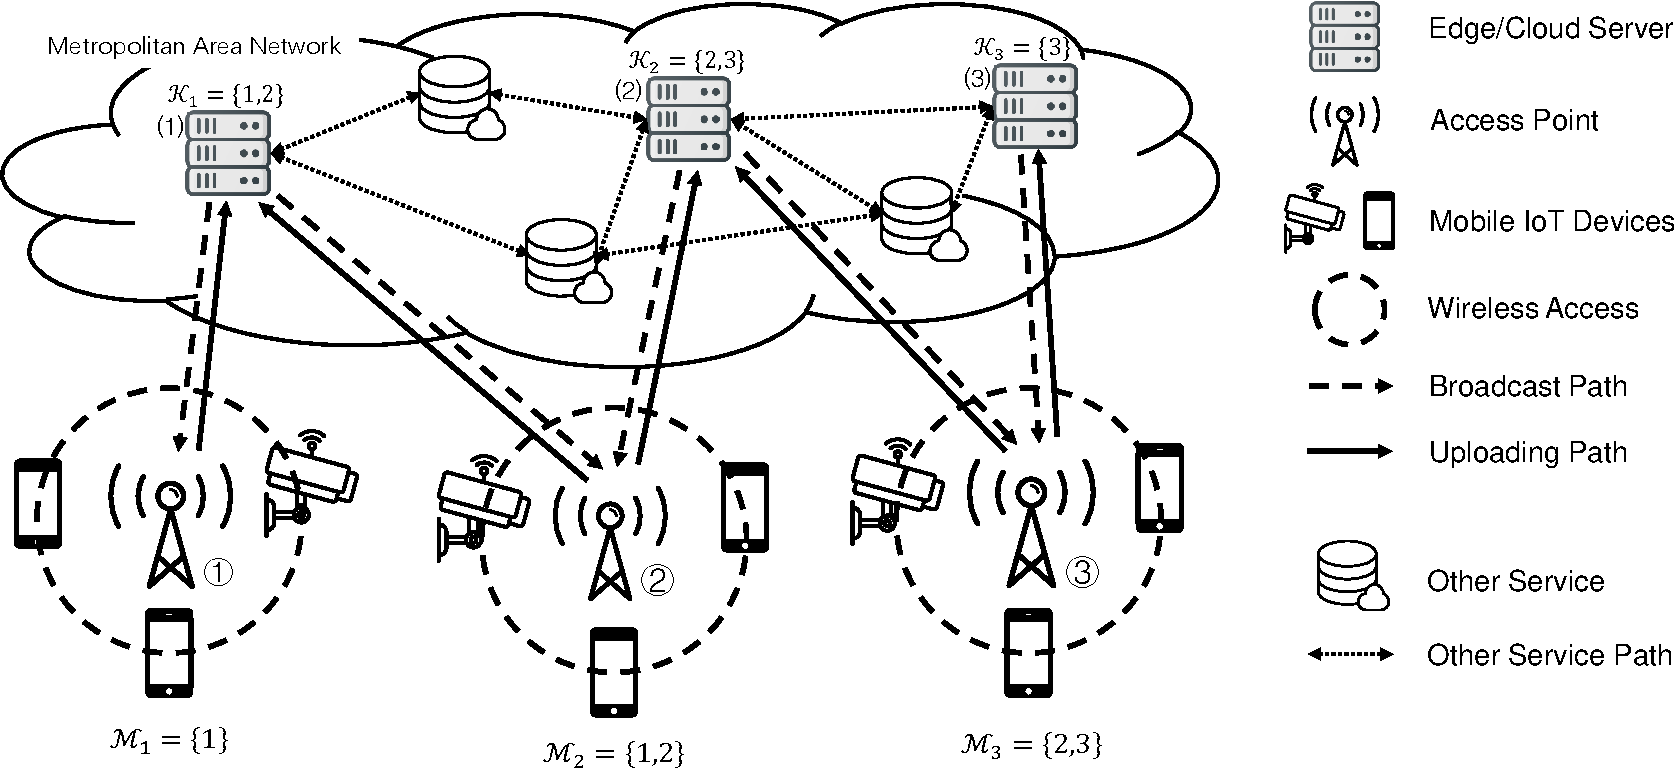
\includegraphics[width=0.60\textwidth]{system-model.pdf}
%     \caption{The Illustration of System Model.}
%     \label{fig:system}
% \end{figure*}
We consider an edge computing system with $K$ Access Points (APs) and $M$ edge servers, which are connected in an edge network as illustrated in Fig.\ref{fig:system}.
The sets of APs and edge servers are denoted as $\apSet \define \set{1,\dots,K}$ and $\esSet \define \set{1,\dots,M}$, respectively.
\hongycCHK{An edge server is typically deployed and collocated with an AP so that mobile devices can upload jobs efficiently.} 
% The communication latency among these APs and edge servers is random.
Each AP collects the computation jobs from the {mobile IoT devices} within its coverage, and makes dispatching \revision{decisions} on the edge servers for each job.
It is assumed that the $k$-th AP only dispatches the computation jobs to the edge servers within a certain number of hops.
Let $\esSet_{k} \subseteq \esSet$ be the subset of edge servers which can compute the jobs from the $k$-th AP, and $\apSet_{m}$ be the subset of APs, which may upload jobs to the $m$-th edge server.
We refer to $\esSet_{k}$ as the \emph{candidate server set} of the $k$-th AP, $\apSet_{m}$ as the \emph{potential AP set} of the $m$-th edge server, \hongycCHK{and $\rho_{k,m}$ as the collocation indicator (i.e., $\rho_{k,m}=1$ if $k$-th AP and $m$-th edge server collocated, otherwise $\rho_{k,m}=0$)} ($\forall k\in\apSet, m\in\esSet$).
Different APs may have different candidate servers according to their locations in the network.%, as illustrated in Fig.\ref{fig:system}.
In this edge computing network, APs and edge servers periodically broadcast their state information (the state information is defined in Section \ref{subsec:broadcast}), and one AP updates its strategy of job dispatching when receiving the broadcast state information.
In this paper, we shall optimize the job dispatching strategy distributed at APs with partially observable state information, where both job uploading and state information broadcasting suffer from random transmission latency.

%NOTE: [job space support and arrival process]
Without loss of generality, it is assumed that there are $J$ types of jobs in this system, which are denoted via the set $\jSpace \define \set{1,\dots,J}$.
The time axis of dispatching is organized by time slots.
The arrivals of the type-$j$ jobs at the $k$-th AP ($\forall k\in\apSet,j\in\jSpace$) in different time slots are assumed to be independent and identically distributed (i.i.d.) Bernoulli random variables, and the arrival probability is denoted as $\lambda_{k,j}$.
Let $B_{k,j}(t) \in \set{0,1}$ represent the event of job arrival, where $B_{k,j}(t)=1$ means one type-$j$ job arrives at the $k$-th AP in the $t$-th time slot, and $B_{k,j}(t)=0$ means otherwise.
Hence,
\begin{align}
    \Pr\{ B_{k,j}(t) = 1 \} = \lambda_{k,j}, \forall t,k\in\apSet,j\in\jSpace.
\end{align}

%NOTE: [uploading process]
Each AP immediately dispatches each type of received jobs to one edge server.
As the APs upload jobs over shared edge networks illustrated in Fig.\ref{fig:system}, the actual uploading time is random due to random traffics initiated from other enabled services.
Moreover, the notification of uploading completion from edge server to AP also consumes random time slots for the same reason, and thus the uploading time is unknown in advance.
Hence, we assume the uploading time of different types of jobs from different APs to edge servers follow independent and discrete distributions.
% \fixit{For the uploading latency of the type-$j$ job from the $k$-th AP to the $m$-th edge server, the other jobs in uploading could be taken as random traffics of other services, and thus the random uploading latency are independent for each job.}
% Different types of jobs may have different distributions of the input data size.
Let $\mathbb{U}_{k,m,j}(\Xi)$ be the uploading latency (in terms of time slots) distribution of the type-$j$ jobs from the $k$-th AP to the $m$-th edge server with support $\set{1, \dots, \Xi}$ ($\forall k\in\apSet, m\in\esSet, j\in\jSpace$), where $\Xi$ is the maximum possible uploading time for all jobs and the expectation is denoted as $u_{k,m,j}$.
\hongycCHK{Specifically, the uploading latency is fixed as $0$ if $\rho_{k,m}=1$ for job uploading to the collocated edge server.}

%NOTE: [computation process]
For job computation process on edge servers, we adopt the \emph{unrelated machines assumption} as in \cite{tan-online} where the computation time on different edge servers would follow independent distributions.
Specifically, there are $J$ parallel virtual machines (VMs) running on each edge server for processing the $J$ job types, respectively.
It is assumed that the computation time of different job types on different edge servers follows independent memoryless geometric distribution 
\footnote{In this paper, we adopt the memoryless geometric distribution to simplify the elaboration of algorithm. In fact, the proposed algorithm can be easily extended to other distributions.}
with different expectations as in \cite{TOWC18-HuangKb}.
Let $\mathbb{G}(1/c_{m,j})$ be the distribution of the computation time slots for the type-$j$ jobs on the $m$-th edge server, where $\mathbb{G}$ denotes the geometric distribution, $c_{m,j}$ is the expectation.
Let $f_{m,j}$ be its probability mass function (PMF), we have
\begin{align}
    f_{m,j}(x) \define (1-\frac{1}{c_{m,j}})^{x-1} \frac{1}{c_{m,j}}, x=1,2,\dots.
\end{align}
For each job type, the uploaded jobs are computed in a First-Come-First-Serve (FCFS) manner, and a processing queue with a maximum job number $L_{max}$ is established for each VM.
The arrival jobs will be discarded when the processing queue is full.

\begin{remark}%[Generalization to Edge-Cloud Model]
    The above network model could be generalized into \revision{a} computing system with both edge servers and cloud center.
    A cloud center could be treated as a special edge server in our model but with stronger computational capability and larger uploading latency and signaling latency \tannCHK{to the APs}.
    % Furthermore, the placement of edge servers in the network determines their latency distributions to the APs in our model.
    % For example, the collocated AP and edge server (i.e., the AP and the edge server are placed at same place) suffers from no or tiny uploading latency and signaling latency between each other.
    % Moreover, the job type assumption could be simply generalized to other edge-cloud model by pre-allocate computation resource for some classified jobs, where resource allocation is not the major concern in this paper.
\end{remark}
%----------------------------------------------------------------------------------------%

\subsection{Signaling Mechanism with Periodic Broadcast}
\label{subsec:broadcast}
In order to facilitate distributed and cooperative dispatching for the APs, {the signaling mechanism with periodic broadcast is introduced.}
We refer to every $t_B$ time slots as a \emph{broadcast interval}.
As illustrated in Fig.\ref{fig:brd_timeline}, at the beginning of each broadcast interval, the local state information (LSI) of APs and edge servers are broadcast, and each AP updates its dispatching strategy of job dispatching when observing the broadcast LSIs from some APs and edge servers.
As a remark notice that the observable LSI may be outdated due to transmission latency among APs and edge servers.
The LSI at the APs and edge servers, global state information, and observable state information at the APs are defined below, respectively.

%NOTE: State and Broadcast Information for AP
\begin{definition}[LSI of APs]
    Let $R^{(k)}_{m,j}(\xi,t,n) \in \set{0,1}$ be the indicator of the type-$j$ jobs at the $n$-th time slot of the $t$-th interval.
    Its value is $1$ when there is one job being uploaded from the $k$-th AP to the $m$-th server which has been delivered for $\xi$ time slots, and $0$ otherwise.
    Let $\omega_{k,j}(t)$ be the target edge server for the type-$j$ jobs of the $k$-th AP at the very beginning of the $t$-th broadcast interval.
    % , and $\omega_{k,j}(t+1)$ be the updated target edge server when the $k$-th AP observes a number of the broadcast LSIs of the $t$-th broadcast interval.
    The LSI of the $k$-th AP at the beginning of the $t$-th broadcast interval is defined as
    {\small
    \begin{align}
        \mathcal{R}_{k}(t) \define
        \Paren{
            \Brace{\vec{R}^{(k)}_{m,j}(t,0) \Big| \forall m\in\esSet,j\in\jSpace},
            \mathcal{A}_{k}(t)
        },
    \end{align}
    }%
    where
    {\small
    \begin{align}
        \vec{R}^{(k)}_{m,j}(t,0) \define \Paren{
            R^{(k)}_{m,j}(0,t,0), \dots, R^{(k)}_{m,j}(\Xi,t,0)
        },
    \end{align}
    }%
    and
    {\small
    \begin{align}
        \mathcal{A}_{k}(t) &\define \Brace{\omega_{k,j}(t) \Big| \forall j\in\jSpace}
    \end{align}
    }%
    are referred as status of the type-$j$ job uploading from the $k$-th AP to the $m$-th edge server, and the dispatching actions for all types of jobs of the $k$-th AP at the beginning of the $t$-th broadcast interval, respectively.
\end{definition}

%NOTE: State and Broadcast Information for Edge Server
\begin{definition}[LSI of Edge Servers]
    Let $Q_{m,j}({t,n})$ be the number of type-$j$ jobs on the $m$-th edge server at the $n$-th time slot of the $t$-th interval ($\forall m\in\esSet, j\in\jSpace$).
    The LSI of the $m$-th edge server in the $t$-th broadcast interval is defined as
    \begin{align}
        \mathcal{Q}_{m}(t) \define \Brace{
            Q_{m,j}(t, 0) \Big| \forall j\in\jSpace
        }.
    \end{align}
\end{definition}

\begin{definition}[Global State Information]
    The global state information (GSI) of the $t$-th broadcast interval is defined as the aggregation of the broadcast LSIs from all the APs and edge servers, i.e.,
    \begin{align}
        \Stat(t) \define
            \Paren{
                \Brace{\mathcal{R}_{k}(t) \Big| \forall k\in\apSet},
                \Brace{\mathcal{Q}_{m}(t) \Big| \forall m\in\esSet}
            }.
    \end{align}
\end{definition}

%NOTE: Conflict of AP set and partial information definition
As the APs and edge servers may reside in different locations of a MAN, the transmission latency of LSI is not negligible.
It might be inefficient {and costly} for one AP to collect the complete GSI before the update of dispatching policy.
For example, the transmission latency of the LSI from the edge servers outside the \emph{candidate server set} $\esSet_{k}$ to the $k$-th AP may be large, and some broadcast information may be discarded by the routers after a certain number of hops.
In this paper, we shall investigate the distributed dispatching design based on the \emph{observable state information} at each AP.
Specifically, the \emph{conflict AP sets} and the \emph{observable state information} are defined below, respectively.
\begin{definition}[Conflict AP Set]
    The conflict AP set to the $k$-th AP ($\forall k\in\apSet$) consists of the neighboring APs who share any common edge server with the $k$-th AP, i.e.,
    \begin{align}
        \ccSet_{k} \define \bigcup_{m\in\esSet_{k}} \apSet_{m}.
    \end{align}
\end{definition}

\begin{definition}[Observable State Information]
    The observable state information (OSI) of the $k$-th AP ($\forall k\in\apSet$) at the $t$-th broadcast interval is defined as the aggregation of LSIs of the APs in {conflict AP set} and the edge servers in {candidate server set} of the $k$-th AP, i.e.,
    {\small
    \begin{align}
        \Stat_{k}(t) &\define
        \Paren{
            \Brace{\mathcal{R}_{k'}(t) \Big| \forall k'\in\ccSet_{k}},
            \Brace{\mathcal{Q}_{m}(t) \Big| \forall m\in\esSet_{k}}
        }.
    \end{align}
    }%
    \label{def:OSI}
\end{definition}

\begin{figure*}[t]
    \centering
    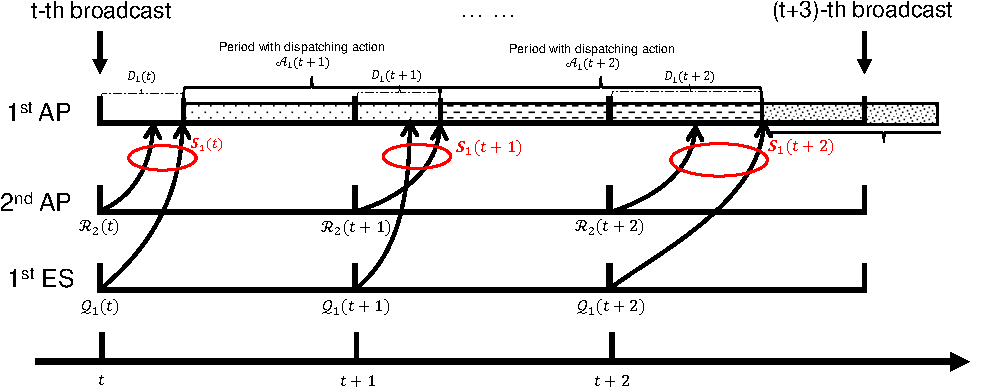
\includegraphics[width=0.60\textwidth]{brd-timeline.pdf}
    \caption{The timeline illustration of reception of OSI for the $1$-st AP where $2$-nd AP is in its \emph{conflict AP set} and $1$-st server is in its \emph{candidate server set}.}
    \label{fig:brd_timeline}
\end{figure*}

The $k$-th AP is able to collect its OSI $\Stat_{k}(t)$ at the $\mathcal{D}_{k}(t)$-th time slots of the $t$-th broadcast interval, where the \emph{\brlatency}~$\mathcal{D}_{k}(t)$ is a random variable.
It is assumed that $\mathcal{D}_{k}(t)$ follows identical and independent distribution in different broadcast interval.
% We refer to $\mathcal{D}_{k}(t)$ as the \brlatency~of the $k$-th AP at the $t$-th broadcast interval.
An example is given below to demonstrate how the \brlatency~affects the reception of OSI and the update of the dispatching strategy.

\begin{example}
    In Fig.\ref{fig:brd_timeline}, the $2$-nd AP and $1$-st server are in the \emph{conflict AP set} and \emph{candidate server set} of the $1$-st AP, respectively.
    At the beginning of the $t$-th broadcast interval, the dispatching actions $\mathcal{A}_{1}(t)$ is adopted by the $1$-st AP.
    After $\mathcal{D}_{1}(t)$ time slots, it updates the dispatching actions to $\mathcal{A}_{1}(t+1)$ based on its OSI $\Stat_{1}(t)$.
    In the $(t+1)$-th broadcast interval, the $1$-st AP will firstly keep the previous actions $\mathcal{A}_{1}(t+1)$, and then updates the actions $\mathcal{D}_{1}(t+1)$ time slots later based on $\Stat_{1}(t+1)$. The new action is denotes as $\mathcal{A}_{1}(t+2)$.
    The signaling latency $\mathcal{D}_1(t)$ and $\mathcal{D}_1(t+1)$ can be different.
\end{example}

\revision{
    \begin{remark}[Handling Broadcast Information Transmission Failure]
        % R1-1: How do you deal with the failed transmission of system state information?
        % R2-2: What if the information broadcast by the 2-nd AP is not received by the 1-st AP?
        The transmission failure of broadcast information could be easily handled with a simple retransmission schema.
        \hongyc{
            In one broadcast interval, if any AP could not receive the broadcast within a certain time limit which is denoted as $\tau_0$ (random variable with support $\set{0, \dots, \hat{\tau}_0}$), it will request a retransmission of the broadcast from the corresponding AP or edge server.
            The AP or edge server will immediately repeat the broadcast when receive the retransmission request, and we denote the Round-Trip Time (RTT) as $\tau_1$ (random variable with support $\set{0, \dots,\hat{\tau}_1}$).
            As the retransmission request or the repeated broadcast may fail again, we denote $\theta_\tau$ as the maximum retransmission times after which the transmission is believed to be received.
            The retransmission times until success is denoted as $\theta_\tau$.
            Therefore, the broadcast interval $T$ must be set to bound the maximum time elapsed $\hat{\theta}_{\tau}(\hat{\tau}_0+\hat{\tau}_1)$ to guarantee the complete reception of OSI in one broadcast interval.
            Moreover, $(\hat{\tau}_0+\hat{\tau}_1)$ is limited because of the original constraint of hops, and $\hat{\theta}_\tau$ is usually small.
            As a remark notice that the elapsed time $\theta_{\tau}(\tau_0+\tau_1)$ for the $k$-th AP at the $t$-th broadcast interval is exactly the \brlatency~$\Delay_k(t)$.
        }
    \end{remark}
}

The notations used throughout this paper are summarized as in Table \ref{table:symbols}.
\begin{table}[htp!]
    % \footnotesize
    \centering
    \caption{Table of notations and their descriptions throughout this paper.}
    \label{table:symbols}
    \begin{tabulary}{0.9\linewidth}{|p{1.8cm}|L|}
        \hline
        Notation                        & Description \\
        \hline
        $\mathcal{K}$                   & The denotation of AP set \\
        $\mathcal{M}$                   & The denotation of edge server set \\
        $\mathcal{K}_{m}$               & The potential AP set of the $m$-th edge server \\
        $\mathcal{M}_{k}$               & The candidate edge server set of the $k$-th AP \\
        $\ccSet_{k}$                    & The conflict AP set of the $k$-th AP  \\
        $\mathcal{J}$                   & The denotation of job types set \\
        $\lambda_{k,j}$                 & The average arrival job rate for the type-$j$ job on the $k$-th AP \\
        $c_{m,j}$                       & The average computation time for the type-$j$ job on the $m$-th edge server \\
        $L_{max}$                       & The maximum job number for each VM \\
        $t_B$                           & The duration of a broadcast interval \\
        $\Xi$                           & The maximum job uploading time \\
        $\xi$                           & The index of time slot of uploading time for one job \\
        $\mathbb{U}_{k,m,j}(\Xi)$       & The uploading latency distribution of the type-$j$ jobs from the $k$-th AP to the $m$-th edge server \\
        $\mathcal{R}_{k}(t)$            & The LSI of the $k$-th AP at the beginning of the $t$-th broadcast interval \\
        $\mathcal{Q}_{m}(t)$            & The LSI of the $m$-th edge server at the beginning of the $t$-th broadcast interval \\
        $D_{k}(t)$                      & The \brlatency~for the $k$-th AP at the $t$-th broadcast interval \\
        $\mathbb{D}(t)$                 & The vector of all \brlatency~ at the $t$-th broadcast interval \\
        $\Stat(t)$                      & The GSI at the $t$-th broadcast interval \\
        $\Stat_{k}(t)$                  & The OSI of the $k$-th AP at the $t$-th broadcast interval \\
        $\omega_{k,j}(t)$               & The dispatching action for type-$j$ job on the $k$-th AP at the beginning of $t$-th broadcast interval \\
        $\mathcal{A}_{k}(t)$               & The dispatching actions of the $k$-th AP at the beginning of $t$-th broadcast interval \\
        $\Policy(\Stat(t),\Delay(t))$   & The aggregation of individual policy all APs \\
        $\Baseline(\Stat(t),\Delay(t))$ & The proposed baseline policy \\
        $\gamma$                        & The discount factor \\
        $\beta$                         & The weight of overflow penalty \\
        $\mathcal{Y}_{n}$               & The $n$-th subset partition in which the APs update their dispatching actions parallelly \\
        $\tilde{\mathcal{A}}(t)$        & The aggregation of dispatching actions of the APs in the subset $\mathcal{Y}_{n}$, where $n \define t \pmod{N}$  \\
        $\hat{\mathcal{A}}(t)$          & The aggregation of dispatching actions of the APs not in the subset $\mathcal{Y}_{n}$, where $n \define t \pmod{N}$ \\
        \hline
    \end{tabulary}
\end{table}